% -------------------------------------------------------------
% SOLUTION(TECHNICAL ASPECT)
% -------------------------------------------------------------
\noindent 

\hspace*{1cm}This chapter outlines the steps undertaken to achieve the final solution, starting from the project description, describing the technical architecture in the process. The development process began with going through the provided Project Description, and rewriting it into a shorter version, keeping only the most important parts. The compact version was suitable for conducting the verb/noun analysis where class and method candidates emerged. The class candidates are able to be transformed into CRC cards outlining the responsibilities and collaborators of each class. The CRC cards are used to provide UML diagrams(Class,Package,Activity and Sequence).

\section{Verb-noun analysis}

\hspace*{1cm}\textcolor{nounred}{Asset Manager (AM)} should \textcolor{verbblue}{store} its \textcolor{nounred}{data} in local \textcolor{nounred}{files} and \textcolor{verbblue}{supply} other \textcolor{nounred}{modules} with it. \textcolor{nounred}{Source Data Manager (SDM)} should \textcolor{verbblue}{store} \textcolor{nounred}{dynamic data} in \textcolor{nounred}{csv files}. \textcolor{nounred}{Result Data Manager (RDM)} should \textcolor{verbblue}{save} \textcolor{nounred}{result data} in local \textcolor{nounred}{CSV files}. \textcolor{nounred}{Optimizer (OPT)} should \textcolor{verbblue}{calculate} the best \textcolor{nounred}{economical schedule} of the \textcolor{nounred}{heat production} for a given \textcolor{nounred}{period}. It also \textcolor{verbblue}{secures} \textcolor{nounred}{heat availability} to all \textcolor{nounred}{buildings} at any \textcolor{nounred}{time}. There are different \textcolor{nounred}{units}, each \textcolor{verbblue}{has} a specific \textcolor{nounred}{production cost}, expressed in \textcolor{nounred}{DKK} per MWh produced \textcolor{nounred}{heat}. For \textcolor{nounred}{heat only units} there are no further \textcolor{nounred}{expenses} nor \textcolor{nounred}{income}. \textcolor{nounred}{Electricity producing units} should \textcolor{verbblue}{sell} the produced \textcolor{nounred}{electricity} and \textcolor{verbblue}{have} thereby an extra \textcolor{nounred}{income} depending on the \textcolor{nounred}{electricity prices} which can \textcolor{verbblue}{change} from \textcolor{nounred}{hour} to \textcolor{nounred}{hour}. \textcolor{nounred}{Electricity consuming units} should \textcolor{verbblue}{buy} the \textcolor{nounred}{electricity} and \textcolor{verbblue}{have} thereby an extra \textcolor{nounred}{expense}, again depending on the \textcolor{nounred}{electricity prices}. \textcolor{nounred}{Net production cost} should be \textcolor{verbblue}{calculated} differently for each \textcolor{nounred}{unit type} and \textcolor{verbblue}{compared} to build \textcolor{nounred}{priorities}. The \textcolor{nounred}{Data Visualization} should \textcolor{verbblue}{display} a \textcolor{nounred}{graphical presentation} of important \textcolor{nounred}{source and result data}.

\vspace{2em}

\subsection*{\textcolor{nounred}{Candidates for classes:}}
\begin{multicols}{3} % splits the list into 3 columns
\begin{itemize}
    \item Asset Manager
    \item Data
    \item Files
    \item Modules
    \item Source Data Manager
    \item Result Data Manager
    \item Optimizer
    \item Schedule
    \item Production
    \item Period
    \item Heat availability
    \item Buildings
    \item Time
    \item Electricity
    \item Units (GB1-EB1)
    \item Income
    \item Expenses
    \item Prices
    \item Net production cost
    \item Unit type
    \item Data Visualization
    \item Presentation
    \item Priorities
\end{itemize}
\end{multicols}

\vspace{2em}

\subsection*{\textcolor{verbblue}{Candidates for methods:}}
\begin{multicols}{3}
\begin{itemize}
    \item Store
    \item Supply
    \item Save
    \item Calculate
    \item Secures
    \item Has
    \item Sell
    \item Have
    \item Depending
    \item Change
    \item Buy
    \item Compare
    \item Display
\end{itemize}
\end{multicols}

\vspace{2em}

\section{Classes and Methods Mapping}
\renewcommand{\arraystretch}{1.5} % adds vertical padding to rows
\begin{tabularx}{\textwidth}{@{} l X @{}}
    \toprule
    \textbf{Class Name} & \textbf{Associated Methods} \\
    \midrule
    \textcolor{nounred}{AssetManager} & \textcolor{verbblue}{store}, \textcolor{verbblue}{supply} \\
    \textcolor{nounred}{SourceDataManager} & \textcolor{verbblue}{store} (dynamic data), \textcolor{verbblue}{read} CSV \\
    \textcolor{nounred}{ResultDataManager} & \textcolor{verbblue}{save} (results) \\
    \textcolor{nounred}{Optimizer} & \textcolor{verbblue}{calculate} (schedule), \textcolor{verbblue}{secure} (heat availability), \textcolor{verbblue}{compare} \\
    \textcolor{nounred}{Unit} & \textcolor{verbblue}{sell} (electricity), \textcolor{verbblue}{buy} (electricity), \textcolor{verbblue}{calculate} net production cost \\
    \textcolor{nounred}{DataVisualization} & \textcolor{verbblue}{display} (graphical data) \\
    \bottomrule
\end{tabularx}

\subsection*{CRC Cards}
% Asset Manager Card
\noindent
\begin{tabularx}{\textwidth}{| X | X |}
    \hline
    \multicolumn{2}{| p{\dimexpr\textwidth-2\tabcolsep-2\arrayrulewidth}|}{\textbf{Class:} \textcolor{nounred}{Asset Manager}} \\
    \hline
    \textbf{Responsibilities} & \textbf{Collaborators} \\
    \hline
    \begin{itemize}[leftmargin=*, nosep, before=\vspace{-0.2\baselineskip}]
        \item Store heater data
    \end{itemize} & 
    \begin{itemize}[leftmargin=*, nosep, before=\vspace{-0.2\baselineskip}]
        \item Optimizer
        \item Data Visualization
        \item Unit
    \end{itemize} \\
    \hline
\end{tabularx}

\vspace{1.5em} % Space between cards

% Optimizer Card
\noindent
\begin{tabularx}{\textwidth}{| X | X |}
    \hline
    \multicolumn{2}{| p{\dimexpr\textwidth-2\tabcolsep-2\arrayrulewidth}|}{\textbf{Class:} \textcolor{nounred}{Optimizer}} \\
    \hline
    \textbf{Responsibilities} & \textbf{Collaborators} \\
    \hline
    \begin{itemize}[leftmargin=*, nosep, before=\vspace{-0.2\baselineskip}]
        \item Calculates heating schedule
    \end{itemize} & 
    \begin{itemize}[leftmargin=*, nosep, before=\vspace{-0.2\baselineskip}]
        \item Asset Manager
        \item Source Data Manager
        \item Result Data Manager
    \end{itemize} \\
    \hline
\end{tabularx}

\vspace{1.5em}

% Source Data Manager Card
\noindent
\begin{tabularx}{\textwidth}{| X | X |}
    \hline
    \multicolumn{2}{| p{\dimexpr\textwidth-2\tabcolsep-2\arrayrulewidth}|}{\textbf{Class:} \textcolor{nounred}{Source Data Manager}} \\
    \hline
    \textbf{Responsibilities} & \textbf{Collaborators} \\
    \hline
    \begin{itemize}[leftmargin=*, nosep, before=\vspace{-0.2\baselineskip}]
        \item Stores market data
    \end{itemize} & 
    \begin{itemize}[leftmargin=*, nosep, before=\vspace{-0.2\baselineskip}]
        \item Optimizer
        \item Data Visualization
    \end{itemize} \\
    \hline
\end{tabularx}

\vspace{1.5em}

% Result Data Manager Card
\noindent
\begin{tabularx}{\textwidth}{| X | X |}
    \hline
    \multicolumn{2}{| p{\dimexpr\textwidth-2\tabcolsep-2\arrayrulewidth}|}{\textbf{Class:} \textcolor{nounred}{Result Data Manager}} \\
    \hline
    \textbf{Responsibilities} & \textbf{Collaborators} \\
    \hline
    \begin{itemize}[leftmargin=*, nosep, before=\vspace{-0.2\baselineskip}]
        \item Save output data
    \end{itemize} & 
    \begin{itemize}[leftmargin=*, nosep, before=\vspace{-0.2\baselineskip}]
        \item Data Visualization
        \item Optimizer
    \end{itemize} \\
    \hline
\end{tabularx}

\vspace{1.5em}

% Data Visualization Card
\noindent
\begin{tabularx}{\textwidth}{| X | X |}
    \hline
    \multicolumn{2}{| p{\dimexpr\textwidth-2\tabcolsep-2\arrayrulewidth}|}{\textbf{Class:} \textcolor{nounred}{Data Visualization}} \\
    \hline
    \textbf{Responsibilities} & \textbf{Collaborators} \\
    \hline
    \begin{itemize}[leftmargin=*, nosep, before=\vspace{-0.2\baselineskip}]
        \item Display important data to the user
    \end{itemize} & 
    \begin{itemize}[leftmargin=*, nosep, before=\vspace{-0.2\baselineskip}]
        \item Source Data Manager
        \item Result Data Manager
        \item Asset Manager
    \end{itemize} \\
    \hline
\end{tabularx}

\vspace{1.5em}

% Units Card
\noindent
\begin{tabularx}{\textwidth}{| X | X |}
    \hline
    \multicolumn{2}{| p{\dimexpr\textwidth-2\tabcolsep-2\arrayrulewidth}|}{\textbf{Class:} \textcolor{nounred}{Units}} \\
    \hline
    \textbf{Responsibilities} & \textbf{Collaborators} \\
    \hline
    \begin{itemize}[leftmargin=*, nosep, before=\vspace{-0.2\baselineskip}]
        \item Contains data for different heaters
        \item Calculate net production costs
    \end{itemize} & 
    \begin{itemize}[leftmargin=*, nosep, before=\vspace{-0.2\baselineskip}]
        \item Optimizer
        \item Asset Manager
    \end{itemize} \\
    \hline
\end{tabularx}

\vspace{2em}

\section{System Design}
\noindent The system design, implementing the five modules(OPT,DV,AM,SDM and RDM), focuses on distinguishing data, services and the presentation layer. This was achieved by storing data in a Database, having a Backend API for services and a Frontend UI for the presentation layer. The layering helps create a modular solution, that is able to implement every module in a logical way, without affecting one another.
\subsection{UML Diagram - Class Diagram}
\begin{figure}[H]
    \centering
    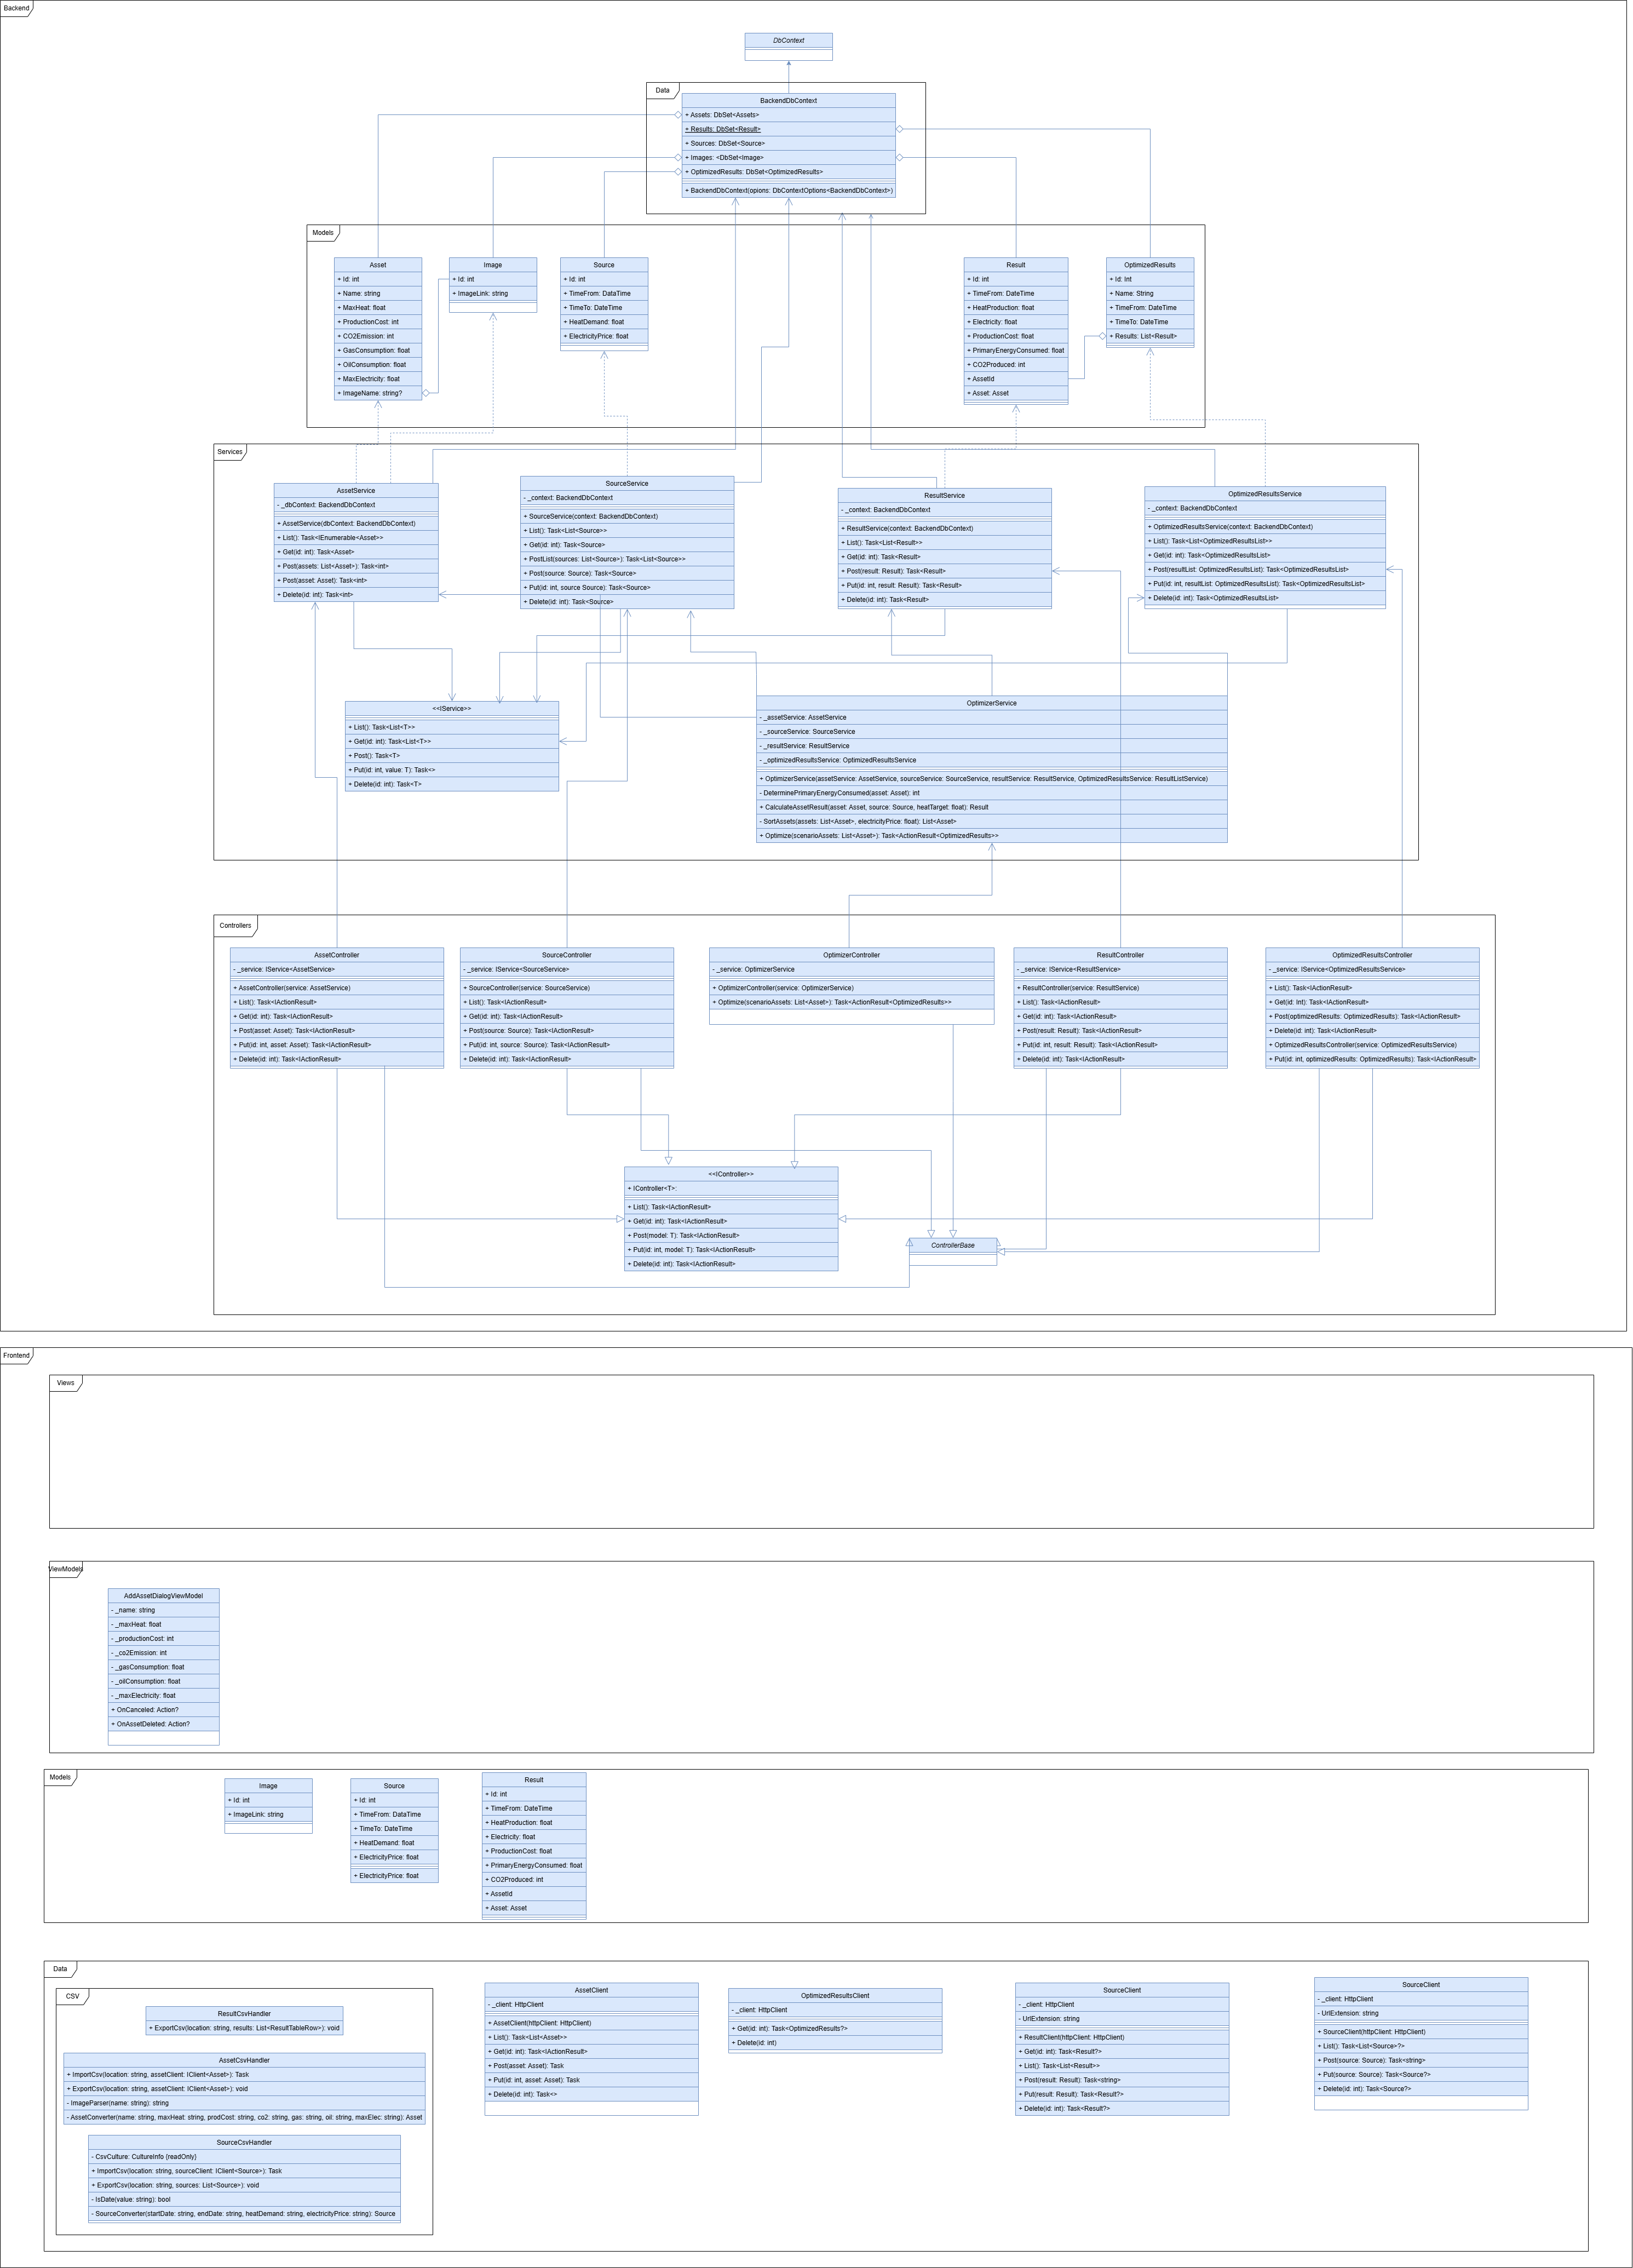
\includegraphics[width=0.9\textwidth]{Images/UML.png} 
    \caption{HeatItOn Abstract Class UML Diagram}
    \label{fig:system_uml}
\end{figure}
\noindent The diagram (Figure~\ref{fig:system_uml}) represents the unified system architecture. This is an abstract version that simplifies the structure down to core components, on which the system is based on. The simplicity of the UML helps with understanding the overall structure of the system, while showing all major classes. 
\subsection{UML Diagram - Package Diagram}
\begin{figure}[H]
    \centering
    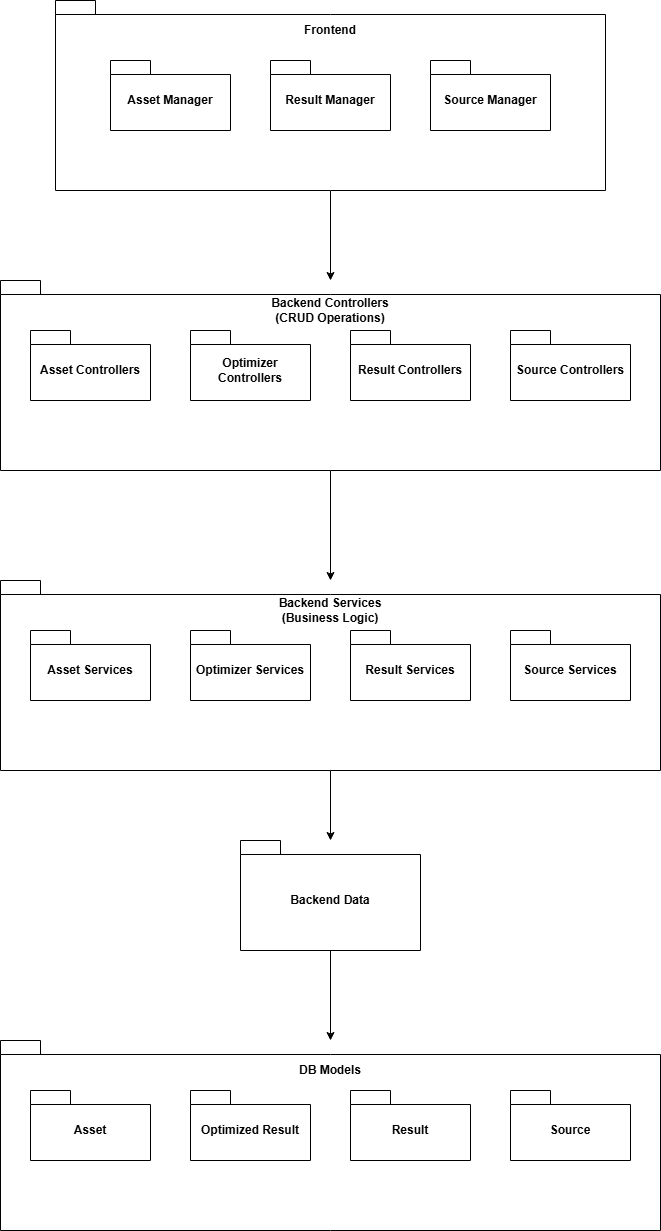
\includegraphics[width=0.8\textwidth]{Images/HeatItOn-Package-Diagram.png} 
    \caption{Package UML Diagram - Five main packages of the system.}
    \label{fig:package_uml}
\end{figure}

The package diagram shown (Figure~\ref{fig:package_uml}) simplified the system into five packages. 

The first one is the Frontend package, containing the Asset, Result and Source Managers. This is the UI of the system, with what the user will interact. The Frontend is following the Model-View-ViewModel pattern, layering the different parts of each manager. This package connects with the next package through clients.

The second package, the Backend Controllers, contain the CRUD(Create, Read, Update, Delete) operations of each module. Through HTTP requests these can be accessed and will call the services in the next package.

Backend Services are the third package containing all the business logic (like the Optimization algorithm).

The forth package is the connection with the Database. It is stored in the Data layer of the Backend. The role of the package is to allow communication between the services and the Database.

The fifth and final package consists of the DB Models(Asset, Source, Result) that are stored in the Database.

This diagram shows a very simplified relationship with the most important parts of the overall system, giving an understanding of the overall workings and layers. Although it is very simple, it is a good starting point for understanding the entire architecture.

The five packages are the backbone of the implementation. Allthough they are much more detailed, this simplified version helps understanding the workings of the solution.

\subsection{UML Diagram - Activity Diagram (Add Asset)}
\begin{figure}[H]
    \centering
    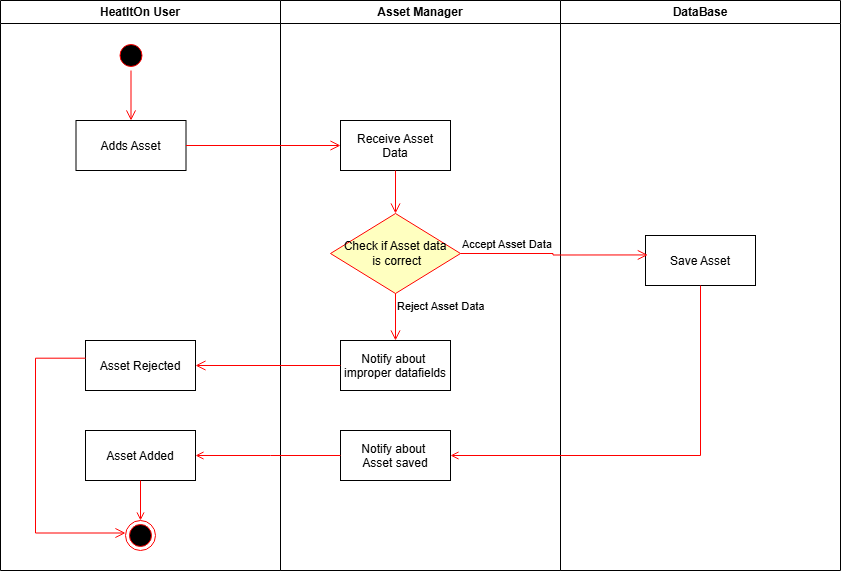
\includegraphics[width=0.9\textwidth]{Images/HeatItOn_activity_diagram_add_asset.png} 
    \caption{Add Asset Activity UML Diagram - Three parts and their actions for adding a new Asset.}
    \label{fig:add_asset_uml}
\end{figure}
The activity UML diagram (Figure~\ref{fig:add_asset_uml}) depicts the addition of a new Asset by the user into the system.

The activity is initiated by the user when they want to add a new Asset interacting with the Asset Manager. The filled out data is then verified by the Asset Manager. If the data was filled out correctly (like having a proper name or number fields having numbers) the Asset Manager will create the Asset and send it to the Database, who will save it. If the data was not filled out correctly, it will reject the received data. The activity ends with the user being notified of both cases, ending it. For a successful addition the Asset Manager will also display the new Asset instantly.

Adding an Asset is started in the Frontend. The Frontend clients will call the Backend that will handle the communication with the Database where the Asset will be saved. The Frontend deals with user input and handling the data as well.

This diagram helps getting an idea about how the communication, for adding Assets, works. This activity is crucial to the solution, as every Asset needs to be stored in the Database for the optimization to work.

\subsection{UML Diagram - Activity Diagram (Import Sources)}
\begin{figure}[H]
    \centering
    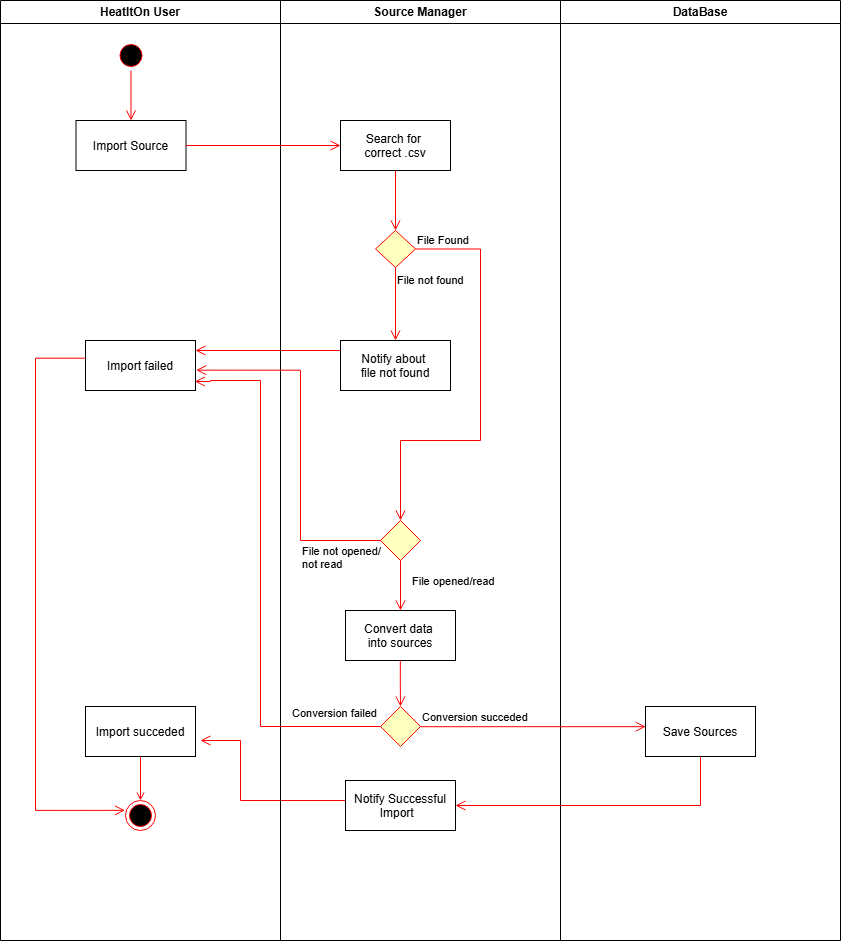
\includegraphics[width=0.9\textwidth]{Images/HeatItOn_activity_diagram_import_source.png} 
    \caption{Import Sources Activity UML Diagram - Three parts and their actions for importing Sources from a csv file.}
    \label{fig:import_sources_uml}
\end{figure}

The activity UML diagram (Figure~\ref{fig:import_sources_uml}) depicts the importing of one or multiple Sources stored in a Comma Separated Value(csv) file. 

Importing is initiated by the user interacting with the Source Manager UI. The Source Manager then will try to find the requested csv file. If the file is found the Source Manager will try to open and read the data in the Frontend. After a successful opening and reading the data will be transformed into proper Source models and will be sent over through the Backend to the Database for storage, notifying the user. If the file is not found or if the file cannot be opened or read properly, like if the csv is not structured properly, the importing process fails and the user is notified. The activity is concluded by notifying the user of either a successful or failed import, the former is visible by a new data set appearing in the Source Manager.

This helps getting an understanding of how importing works for sources (but not only), and the workings of the Source Manager.

The Source Manager and Sources are the other crucial part of the system, without which, the optimization process could not be run.

\subsection{UML Diagram - Activity Diagram (Delete Asset)}
\begin{figure}[H]
    \centering
    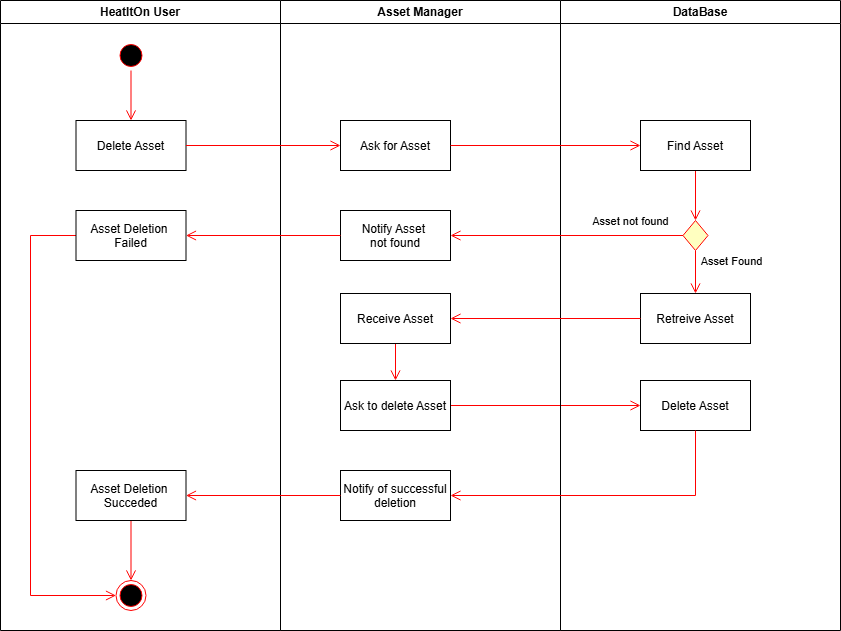
\includegraphics[width=0.9\textwidth]{Images/HeatItOn_activity_diagram_delete_asset.png} 
    \caption{Delete Asset Activity UML Diagram - Three parts and their actions for deleting Assets.}
    \label{fig:delete_assets_uml}
\end{figure}

The activity UML diagram (Figure~\ref{fig:delete_assets_uml}) depicts the deletion of an Asset through the Asset Manager.

Deletion is initiated by the user through interacting with the Asset Manager UI. The Asset Manager will try to retrieve the Asset from the Database(through the Backend). If the Database finds the Asset it will return it to the Asset Manager. If the Database could not find the requested Asset, it will prompt the Asset Manager to notify the user ending the activity. If the Asset is found it will be retrieved to the Asset Manager who will request its deletion from the Database. The Database deletes the Asset and the Manager will notify the user of the activity being successful, after which it ends.

This activity diagram portrays another CRUD operation, in this case Deletion, in the system.

This helps getting an understanding of how deletion of objects works in the system, using Assets as an
example. Deletion is crucial for the proper workings of the system.

Deletion is used with Assets, as seen on the diagram, but also with Results, where the user has the option to delete either of them.

\subsection{UML Diagram - Activity Diagram (Optimize)}
\begin{figure}[H]
    \centering
    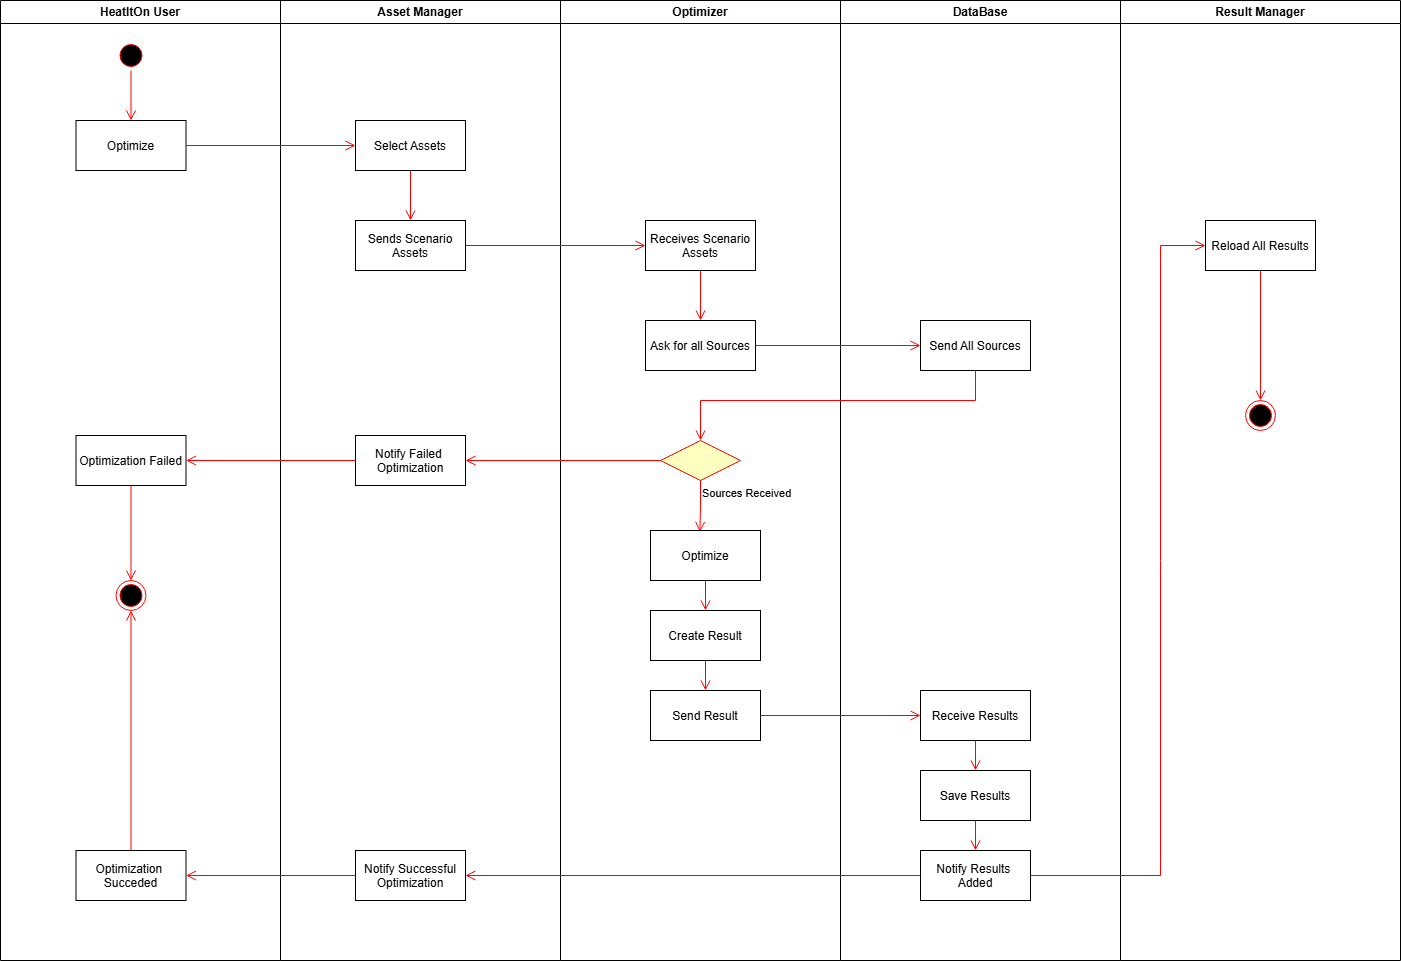
\includegraphics[width=0.9\textwidth]{Images/HeatItOn_activity_diagram_optimize.png} 
    \caption{Optimization Activity UML Diagram - Three parts and their actions for deleting Assets.}
    \label{fig:optimization_uml}
\end{figure}

The activity UML diagram (Figure~\ref{fig:optimization_uml}) depicts the optimization process.

First, the optimization starts with the user, using the Asset Manager UI, selecting Assets and starting the optimization process. The Asset Manager will send the selected Assets to the Optimization module, which after receiving them, will call from the Database all stored Sources up to that moment. If no Source is received it will prompt the Asset Manager to notify the user and end the activity. The Optimizer has no UI elements and is completely in the Backend. If it receives Sources, it will run the optimization algorithm, which will create a Result. The new Result is sent and stored in the Database that will notify both the Asset Manager(that in turn notifies the user) and the Result Manager that there is a new Result ready to be displayed, ending the activity.

This activity diagram proves its relevancy by demonstrating the optimization activity, which is the entire purpose of the system. While it is not enough for a full understanding of the optimization process, the diagram illustrates the different overall steps happening.

Optimization is the part that interacts with every module of the system. It uses directly or indirectly every implemented Manager, and all the activity diagrams(and all their depicted actions) are just helping the optimization process depicted here.

\subsection{UML Diagram - Sequence Diagram (Optimize)}

\begin{figure}[H]
    \centering
    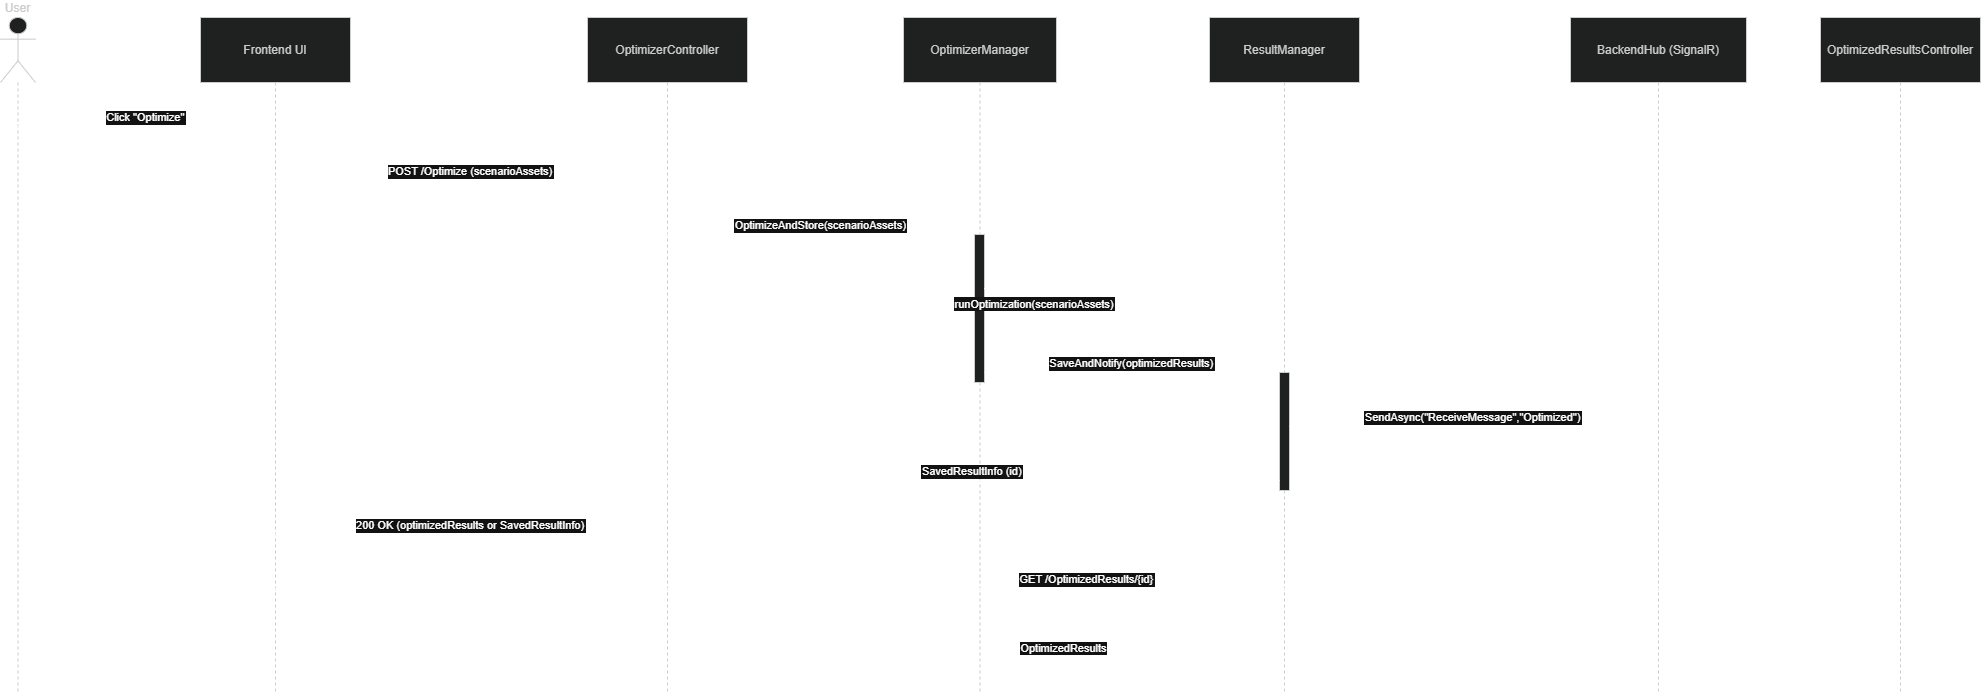
\includegraphics[width=0.9\textwidth]{Images/Sequence_diagram_optimize.drawio.png}
    \caption{Sequence UML diagram of optimization process}
    \label{fig:optimization_sequence}
\end{figure}

\hspace*{1cm}The sequence UML diagram (Figure~\ref{fig:optimization_sequence}) depicts the optimization process. The participants are: User, Frontend UI, `OptimizerController`, `OptimizerManager` (runs the algorithm), `ResultManager` (saves results and sends notifications), `BackendHub` (SignalR) and `OptimizedResultsController` (for later retrieval). The flow is: the user clicks Optimize in the frontend, the frontend sends the selected assets to `OptimizerController` with `POST /Optimize`, `OptimizerController` calls `OptimizerManager` to run the optimization, `OptimizerManager` produces an `OptimizedResults` object and gives it to `ResultManager` to save, `ResultManager` writes the result to the database and asynchronously notifies clients via `BackendHub.SendAsync("ReceiveMessage","Optimized")`, the controller returns either the full result or a small confirmation (`SavedResultInfo` with the new id) to the frontend, the frontend can then request the stored result with `GET /OptimizedResults/{id}` from `OptimizedResultsController` to display the full persisted data. If the optimizer cannot find required source data, it returns an error/notification back to the frontend and the activity ends with the user being informed. In the diagram the `OptimizerManager` and `ResultManager` are shown as manager boxes that group the backend logic (they represent the real services and saving/notification steps) so the sequence stays easy to read while matching the actual system behavior. 

This sequence diagram shows the main flow: how a user action becomes an optimized schedule and is delivered to the UI, connecting the user, backend computation, storage and real-time updates so the reader sees the end-to-end behavior without needing the algorithm details.

How this maps to the code:

\begin{itemize}
    \item The optimizer endpoint is in OptimizerController, the OptimizerController receives the POST /Optimize request.
    \item The optimization work runs in OptimizerService (this is the diagram’s OptimizerManager).
    \item Saving the results is done by OptimizedResultsService (the diagram’s ResultManager).
    \item Real-time notifications go through SignalR in BackendHub, controllers use IHubContext<BackendHub>.SendAsync to send messages.
    \item Fetching stored results is handled by OptimizedResultsController.
    \item The database model and migrations are in BackendDbContext.
    \item Centralized error handling (turning exceptions into HTTP responses) is implemented in ExceptionHandlingMiddleware.
\end{itemize}

\subsection{UML Diagram - Sequence Diagram (Refresh)}

\begin{figure}[H]
    \centering
    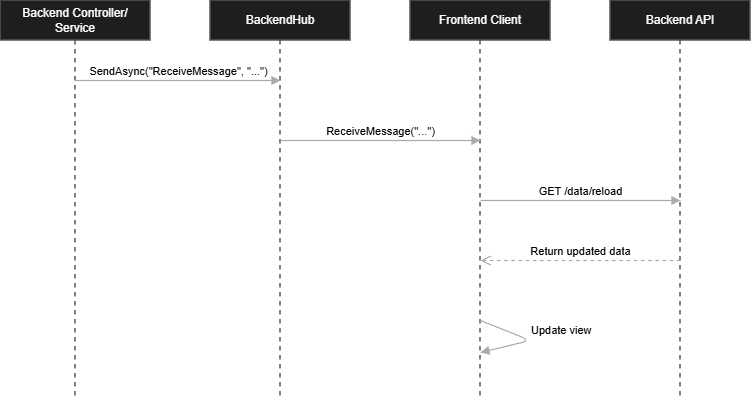
\includegraphics[width=0.9\textwidth]{Images/Sequence_diagram_refresh.png}
    \caption{Sequence UML diagram of refreshing process}
    \label{fig:refresh_sequence}
\end{figure}

\hspace*{1cm}The refresh sequence diagram is relevant because it shows how the frontend stays synchronized with changes made in the backend, which is an important part of the system’s behavior. It demonstrates the full update flow after a backend action has changed some data: the backend first sends a SignalR notification and then the frontend reacts by loading the latest data again. This makes the diagram useful because it explains how the user sees updated information without manually reloading the page and it also shows the difference between pushing a notification and pulling the new data. The diagram connects directly to the implemented solution in the codebase: controllers and services use `IHubContext<BackendHub>` to call `SendAsync(...)`, the frontend receives the `ReceiveMessage` event and then it requests the updated data from the backend through endpoints such as `OptimizedResultsController` or another reload request. In this way, the diagram reflects the real implementation and shows how real-time updates are handled in the system.
\section{System Technical Architecture}

\hspace*{1cm}For the system architecture, from a technical standpoint, C\# \cite{csharp} was chosen as the base technology stack. This was chosen as its .NET 9.0 version is suitable for the development of this system with its simplicity, the familiarity of the team and its object-oriented imperative style. Every other piece of technology is related to .NET and was chosen based on their respective compatibility with the language.

\subsection*{Technology Stack}

\hspace*{1cm}The first chosen piece was the Database that is running MySQL \cite{dubois2013mysql}. The role of the Database is to store the system data independently from other parts of the system(Backend and Frontend). It stores relevant user data, using models, like the Assets, Sources, Results of each generator and Results of optimization runs. The Database communicates with the Backend using MicrosoftEntityFramework. The Frontend cannot communicate directly with the Database, it must do it through the Backend. The Database allows data storage that is independent from runs. The system can work with multiple users at the same time or with one user in different runs, storing all the data in the Database, where it will remain until deletion.
 
The second chosen piece of technology stack is for the Frontend UI. For this AvaloniaUI was chosen for its good compatibility with .NET and modularity. Besides this, the Frontend is following the Model-View-ViewModel (MVVM) design pattern.

\subsection*{Layering}

\hspace*{1cm}The system is divided into three main parts, Frontend, Backend and the Database. Each serves a different role and, besides the Database, they are further separated for proper readability and modularity.

The Frontend, as stated earlier, follows the MVVM pattern. The Models, together with the Data (containing file I/O and clients) form the overall data and business layer. The View forms the presentation layer, containing all the UI elements. The ViewModel creates a connection layer between the two other parts. 

The Backend is following a .NET web application template. Its role is to create a connection between the Frontend and Database with an Application Programming Interface (API), and to handle overall business logic for the entire system. For modularity, this is achieved through serious layering. The Backend consists of six main parts. Controllers handle incoming/outgoing traffic to/from the Database and Frontend and will call the appropriate Services. Services contain all the business logic of the system(like optimization or add Asset). Both Controllers and Services inherit from two Interfaces, as they share similarities (like CRUD operations). The Data layer is composed of two other parts, Models(storing data models) and Data(storing DB Migrations and DB Context which is the main connection point to the DB). The presentation layer is completed by the last element, Hubs, which ensures real time communication with the Frontend application (instantly notifies to refresh the Frontend). Although the Backend is divided into many pieces, this was necessary for modularity, readability and because of complexity as well. This way each small section is responsible of one part, making replacement easier. In this solution, if one wants to hypothetically change the entire optimization algorithm, they only need to rework the Optimization Service, without having to touch any other parts.

\subsection*{Architectural Style}

\hspace*{1cm}The implementation follows multiple coding and design principles. The main set of principles that the project adheres to, is SOLID. This happens in both Frontend and Backend and is visible in many parts, like interfaces or being able to add new features without having to change code. SOLID principles help create an Object-Oriented design. But besides these, the project follows DRY (Do not Repeat Yourself), KISS  (Keep It Simple, Stupid), YAGNI (You Aren't Gonna Need It) and SoC (Separation of Concerns).

The technology stack, the layering and the architectural style used are all necessary for the proper running of the system. While the technology stack was kept simple by only using what was necessary for achieving requirements, the layering and style help build a good quality project that is easy to understand, change and complete. But extensive layering also helps following the style, by breaking up the large task into small sections creating a \textit{Divide et impera} style of development, making it easier to adhere to the principles.  


